\documentclass[12pt, a4paper]{report}

\usepackage[unicode	]{hyperref}
\hypersetup{
	colorlinks=false, %set true if you want colored links
	linktoc=all,     %set to all if you want both sections and subsections linked
	linkcolor=black,  %choose some color if you want links to stand out
	filecolor=black,      
	urlcolor=black,
}
\usepackage{cmap} % Улучшенный поиск русских слов в полученном pdf-файле
\usepackage[T2A]{fontenc} % Поддержка русских букв
\usepackage[utf8]{inputenc} % Кодировка utf8
\usepackage[english,russian]{babel} % Языки: английский, русский
\usepackage{enumitem}


\usepackage{threeparttable}

\usepackage[14pt]{extsizes}

\usepackage{caption}
\usepackage{pdfpages}
\usepackage{enumitem}
\renewcommand*\labelenumi{\theenumi)}
\usepackage{float}
\captionsetup{labelsep=endash}
\usepackage{geometry}
\geometry{left=30mm}
\geometry{right=10mm}
\geometry{top=20mm}
\geometry{bottom=20mm}
\usepackage[justification=centering]{caption} % Настройка подписей float объектов
\usepackage{titlesec}
\titleformat{\section}
{\normalsize\bfseries}
{\thesection}
{1em}{}
\titlespacing*{\chapter}{0pt}{-30pt}{8pt}
\titlespacing*{\section}{\parindent}{*4}{*4}
\titlespacing*{\subsection}{\parindent}{*4}{*4}

\usepackage{setspace}
\onehalfspacing % Полуторный интервал

\frenchspacing
\usepackage{indentfirst} % Красная строка

\usepackage{titlesec}
\titleformat{\chapter}{\Large\bfseries}{\thechapter}{20pt}{\Large\bfseries}
\titleformat{\section}{\Large\bfseries}{\thesection}{20pt}{\Large\bfseries}
\newcommand{\centerchapter}[1]{\titleformat{\chapter}{\filcenter\Large\bfseries}{\thechapter}{20pt}{}\addcontentsline{toc}{chapter}{#1}\chapter*{#1}}
\newcommand{\averchapter}[1]{\titleformat{\chapter}{\Large\bfseries}{\thechapter}{20pt}{}\chapter{#1}}
\usepackage{graphicx}
\usepackage{amsmath}
\usepackage{listings}
\usepackage{svg}
\usepackage{setspace}
\onehalfspacing
\usepackage{titlesec}
\titleformat{\section}
{\normalsize\bfseries}
{\thesection}
{1em}{}
\titlespacing*{\chapter}{0pt}{-30pt}{8pt}
\titlespacing*{\section}{\parindent}{*4}{*4}
\titlespacing*{\subsection}{\parindent}{*4}{*4}
\usepackage{titlesec}
\titleformat{\chapter}{\LARGE\bfseries}{\thechapter}{20pt}{\LARGE\bfseries}
\titleformat{\section}{\Large\bfseries}{\thesection}{20pt}{\Large\bfseries}
\newcommand*{\chapterformat}{%
	\mbox{\chapappifchapterprefix{\nobreakspace}\thechapter\autodot\enskip}%
}
\usepackage{xcolor}
\definecolor{codegreen}{rgb}{0,0.6,0}
\definecolor{codegray}{rgb}{0.5,0.5,0.5}
\definecolor{codepurple}{rgb}{0.58,0,0.82}
\definecolor{backcolour}{rgb}{0.95,0.95,0.92}
\lstdefinestyle{mystyle}{
    numberstyle=\tiny\color{codegray},
    basicstyle=\ttfamily\footnotesize,
    breakatwhitespace=false,         
    breaklines=true,                 
    captionpos=t,                    
    keepspaces=true,                 
    numbers=left,                    
    numbersep=5pt,                  
    showspaces=false,                
    showstringspaces=false,
    showtabs=false,                  
    tabsize=2
}
\lstset{style=mystyle}
\usepackage{caption}


\begin{document}
\renewcommand{\contentsname}{Содержание}
\begin{titlepage}
	\newgeometry{pdftex, left=2cm, right=2cm, top=2.5cm, bottom=2.5cm}
	\fontsize{12pt}{12pt}\selectfont
	\noindent \begin{minipage}{0.15\textwidth}
		
\includegraphics[width=\linewidth]{img/b_logo.jpg}
	\end{minipage}
	\noindent\begin{minipage}{0.9\textwidth}\centering
		\textbf{Министерство науки и высшего образования Российской Федерации}\\
		\textbf{Федеральное государственное бюджетное образовательное учреждение высшего образования}\\
		\textbf{«Московский государственный технический университет имени Н. Э.~Баумана}\\
		\textbf{(национальный исследовательский университет)»}\\
		\textbf{(МГТУ им. Н. Э.~Баумана)}
	\end{minipage}
	
	\noindent\rule{18cm}{3pt}
	\newline\newline
	\noindent ФАКУЛЬТЕТ $\underline{\text{«Информатика и системы управления»~~~~~~~~~~~~~~~~~~~~~~~~~~~~~~~~~~~~~~~~~~~~~~~~~~~~~~~}}$ \newline\newline
	\noindent КАФЕДРА $\underline{\text{«Программное обеспечение ЭВМ и информационные технологии»~~~~~~~~~~~~~~~~~~~~~~~}}$\newline\newline\newline\newline\newline\newline\newline
	
	
	
	\begin{center}
		\Large\textbf{Отчет по лабораторной работе № 1} \\
		\Large\textbf{по курсу «Анализ алгоритмов»}
	\end{center}
	\vfill
	
	\noindent\textbf{Тема} $\underline{\text{~~Расстояние Левенштейна и Дамерау-Левенштейна~~~~~~~~~~~~~~~~~~~~~~~~~~~~~~~~~~~~~~~~~~~}}$\newline\newline
	\noindent\textbf{Студент} $\underline{\text{~~Маслюков П.В.~~~~~~~~~~~~~~~~~~~~~~~~~~~~~~~~~~~~~~~~~~~~~~~~~~~~~~~~~~~~~~~~~~~~~~~~~~~~~~~~~~~~~~~~~}}$\newline\newline
	\noindent\textbf{Группа} $\underline{\text{~~ИУ7-52Б~~~~~~~~~~~~~~~~~~~~~~~~~~~~~~~~~~~~~~~~~~~~~~~~~~~~~~~~~~~~~~~~~~~~~~~~~~~~~~~~~~~~~~~~~~~~~~~~~}}$\newline\newline
	\noindent\textbf{Оценка (баллы)} $\underline{\text{~~~~~~~~~~~~~~~~~~~~~~~~~~~~~~~~~~~~~~~~~~~~~~~~~~~~~~~~~~~~~~~~~~~~~~~~~~~~~~~~~~~~~~~~~~~~~~~~~~~}}$\newline\newline
	\noindent\textbf{Преподаватель} $\underline{\text{~~Волкова Л. Л.~~~~~~~~~~~~~~~~~~~~~~~~~~~~~~~~~~~~~~~~~~~~~~~~~~~~~~~~~~~~~~~~~~~~~~~~~~~~~~}}$\newline
	
	\begin{center}
		\vfill
		Москва~---~\the\year
		~г.
	\end{center}
	\restoregeometry
\end{titlepage}


\setcounter{page}{2}
\tableofcontents
\centerchapter{Введение}
\hspace{\parindent}
Задачу ускорения обработки данных можно решить с помощью введение конвейерной обработки. Вводится конвейерная лента и обрабатывающие устройства. Данные поступают на обрабатывающее устройство, которое после завершения обработки передает их дальше по ленте, и не ожидая завершения цикла, приступает к обработке следующих  данных.   

\hspace{\parindent}
Целью работы является исследование конвейерной обработки данных.

\hspace{\parindent}
Задачи, которые необходимо выполнить:
\begin{enumerate}
	\item описать и реализовать алгоритм конвейерной обработки данных;
	\item реализовать алгоритм линейной обработки данных;
    \item провести тестирование по времени для этих алгоритмов;
    \item провести сравнительный анализ по времени для этих алгоритмов.
\end{enumerate}
\chapter{Аналитическая часть}

В данном разделе будут описаны алгоритмы сортировки выбором, бусинами и блочной сортировки.

\section{Сортировка выбором}

Сортировка выбором состоит из следующих шагов:

\begin{itemize}
	\item выбирается элемент неотсортированной части последовательности с наименьшим значением;
	\item выбранный элемент меняется местами с элементом, стоящим на первой позиции в неотсортированной части. Обмен не нужен, если это и есть минимальный элемент;
	\item повтор шагов 1 и 2 до тех пор, пока не останется только наибольший элемент.
\end{itemize}

\section{Блочная сортировка}

Алгоритм сортировки, который работает путем распределения элементов массива по нескольким сегментам. Затем каждый сегмент сортируется индивидуально, либо с использованием другого алгоритма сортировки, либо путем рекурсивного применения блочной сортировки.

Алгоритм работает следующим образом.
\begin{itemize}
	\item Пусть $l$ – минимальный, а $r$ – максимальный элемент массива. Разобьем элементы на блоки, в первом будут элементы от $l$ до $l + k$, во втором – от $l + k$ до $l + 2k$ и т.д., где $k = (r$ – $l) / \textup{количество блоков}$.
	\item Все получившиеся блоки сортируются другим алгоритмом сортировки.
	\item Выполняется слияние блоков в единый массив.
\end{itemize}

\section{Сортировка бусинами}

Алгоритм сортировки  бусинами, работает путем создания матрицы и последующего распределения элементов исходного массива. Каждое число записывается количество раз равное самому числу. Затем матрица трансплонируется и подсчитывается количество вхождений. Таким образом мы получаем отсортированный числа исходного массива \cite{beads}.

Метод ограничен, прежде всего применим к натуральным числам, т.е. можно сортировать только положительные числа. 
Можно сортировать и целые, но это запутаннее - отрицательные числа придется обрабатывать отдельно отрицательные от положительных.


\section*{Вывод}

Были рассмотрены следующие алгоритмы сортировки: выбором, бусинами и блочная. 
Для указанных алгоритмов необходимо получить теоретическую оценку и доказать её экспериментально.
\chapter{Конструкторская часть}

В данном разделе будут представлены схемы алгоритмов: полного перебора и муравьиного алгоритма. Будут описаны типы и структуры данных, используемые для реализации.

\section{Разработка алгоритмов}

На рисунке \ref{img:brute} приведена схема алгоритма решения задачи коммивояжера полным перебором. Схемы муравьиного алгоритма приведена на рисунке \ref{img:ant}, вспомогательные функции данного алгоритма показаны на рисунках \ref{img:choose}-\ref{img:update}.

\begin{figure}[H]
	\begin{center}
		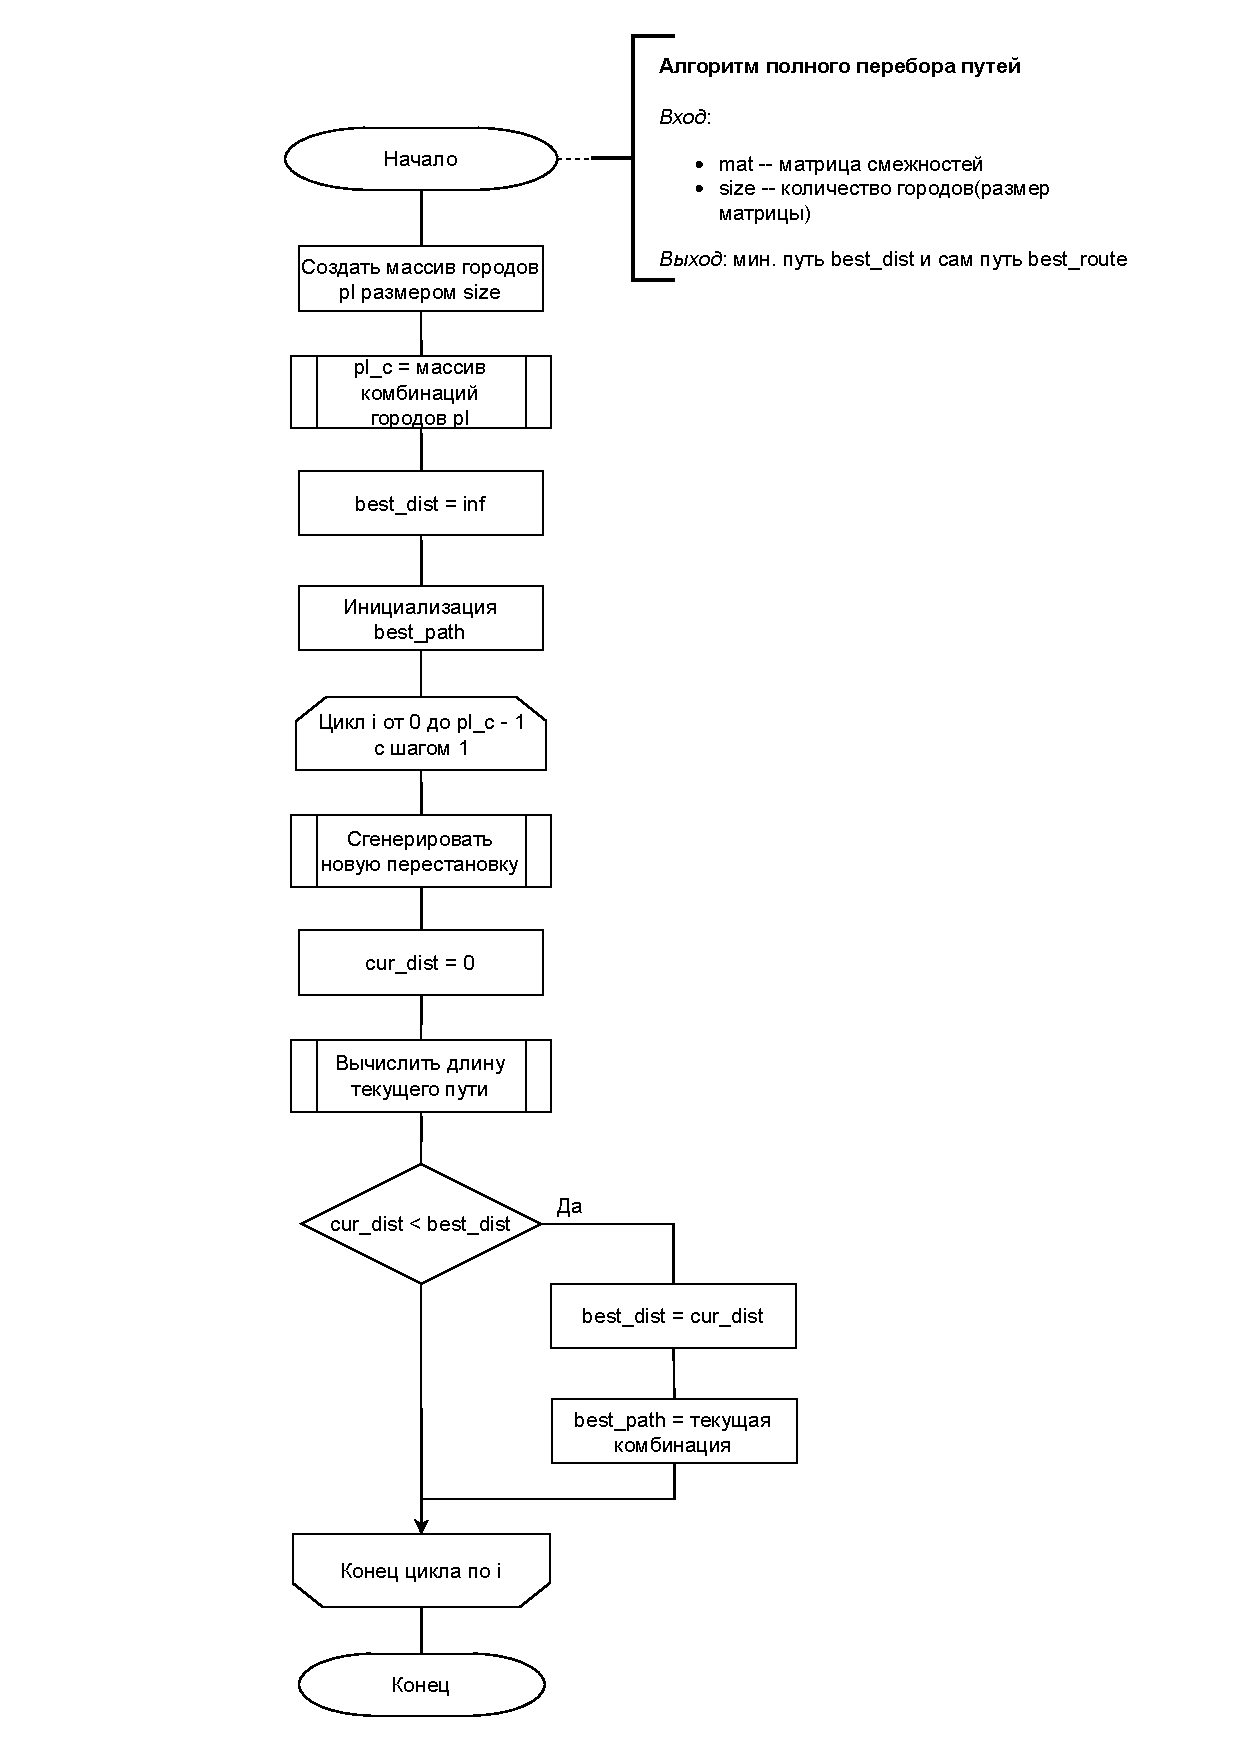
\includegraphics[scale=0.6]{img/brute_force.pdf}
	\end{center}
	\captionsetup{justification=centering}
	\caption{Полный перебор}
	\label{img:brute}
\end{figure}

\begin{figure}[H]
	\begin{center}
		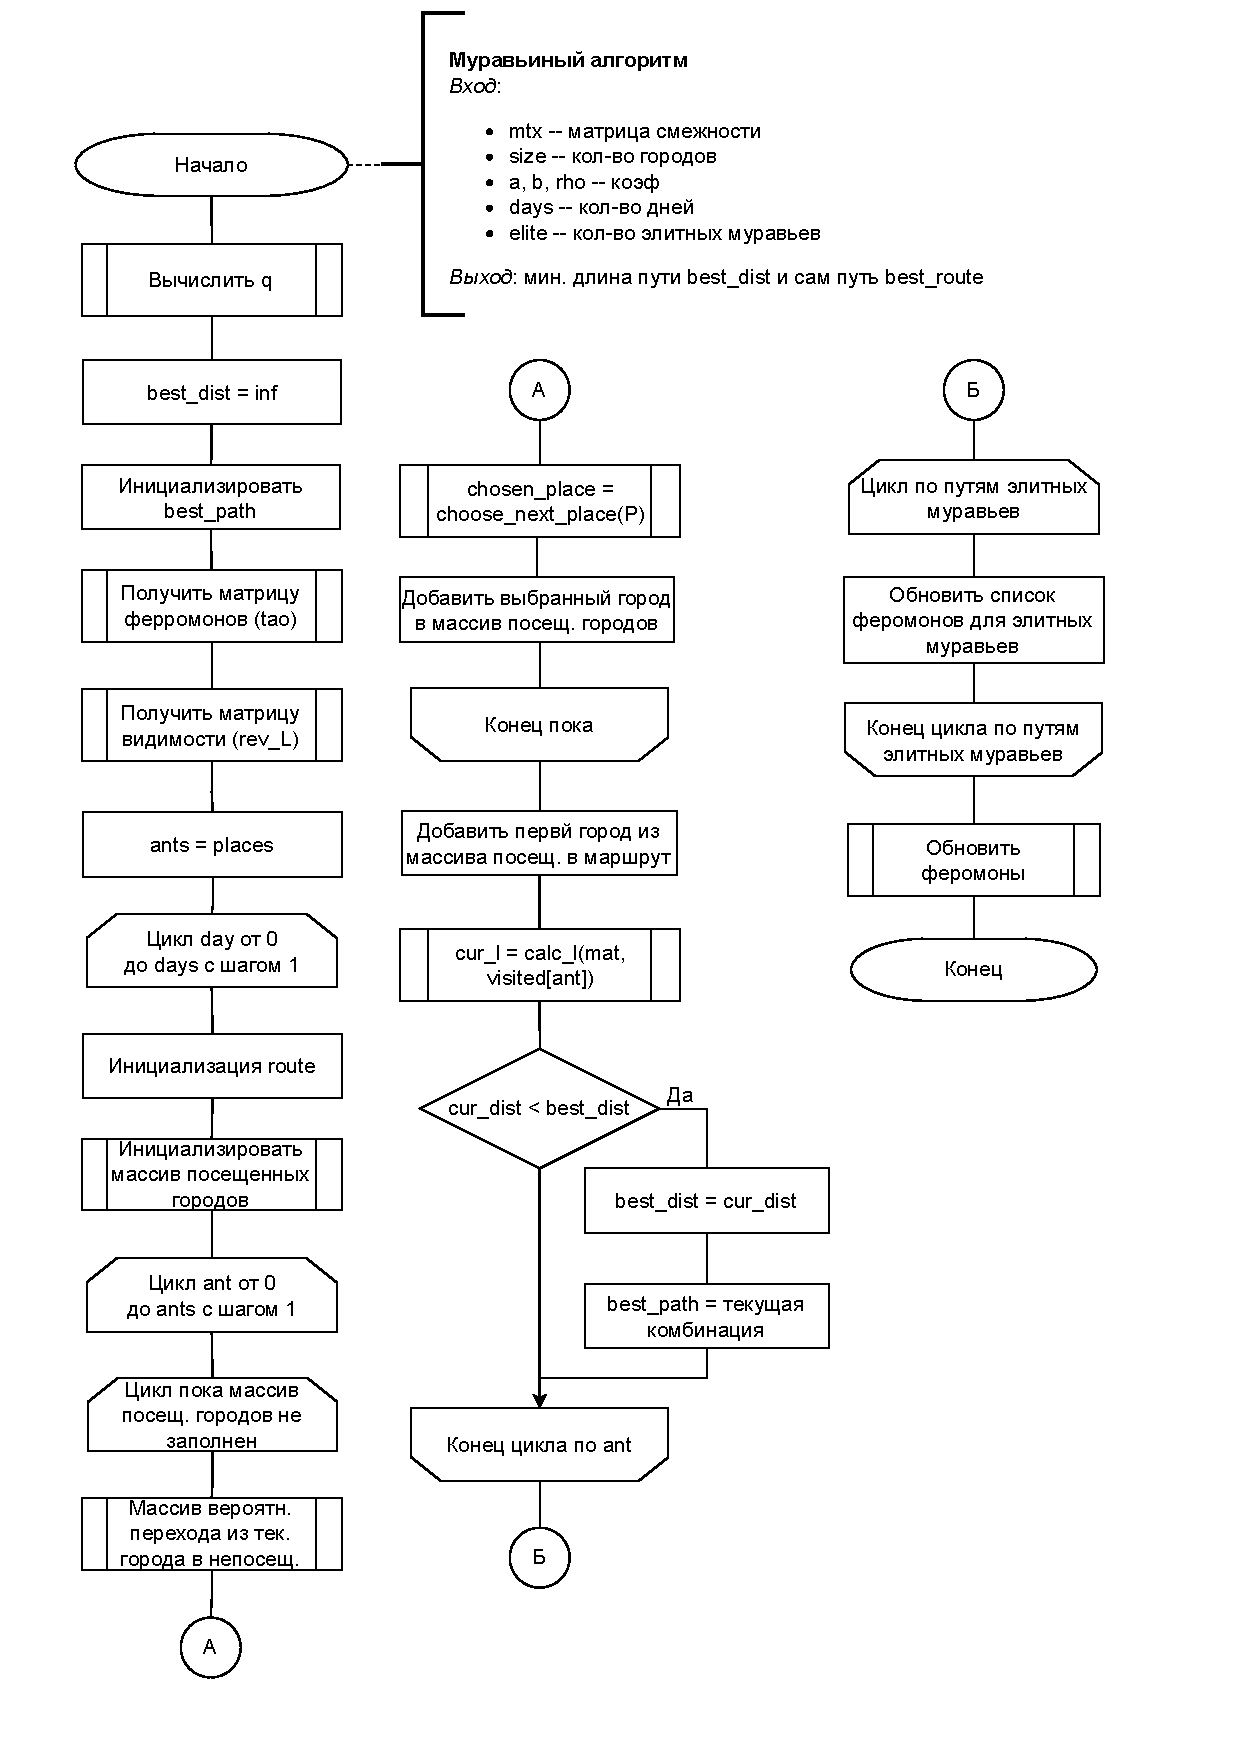
\includegraphics[scale=0.7]{img/ants.pdf}
	\end{center}
	\captionsetup{justification=centering}
	\caption{Муравьиный алгоритм}
	\label{img:ant}
\end{figure}


\begin{figure}[H]
	\begin{center}
		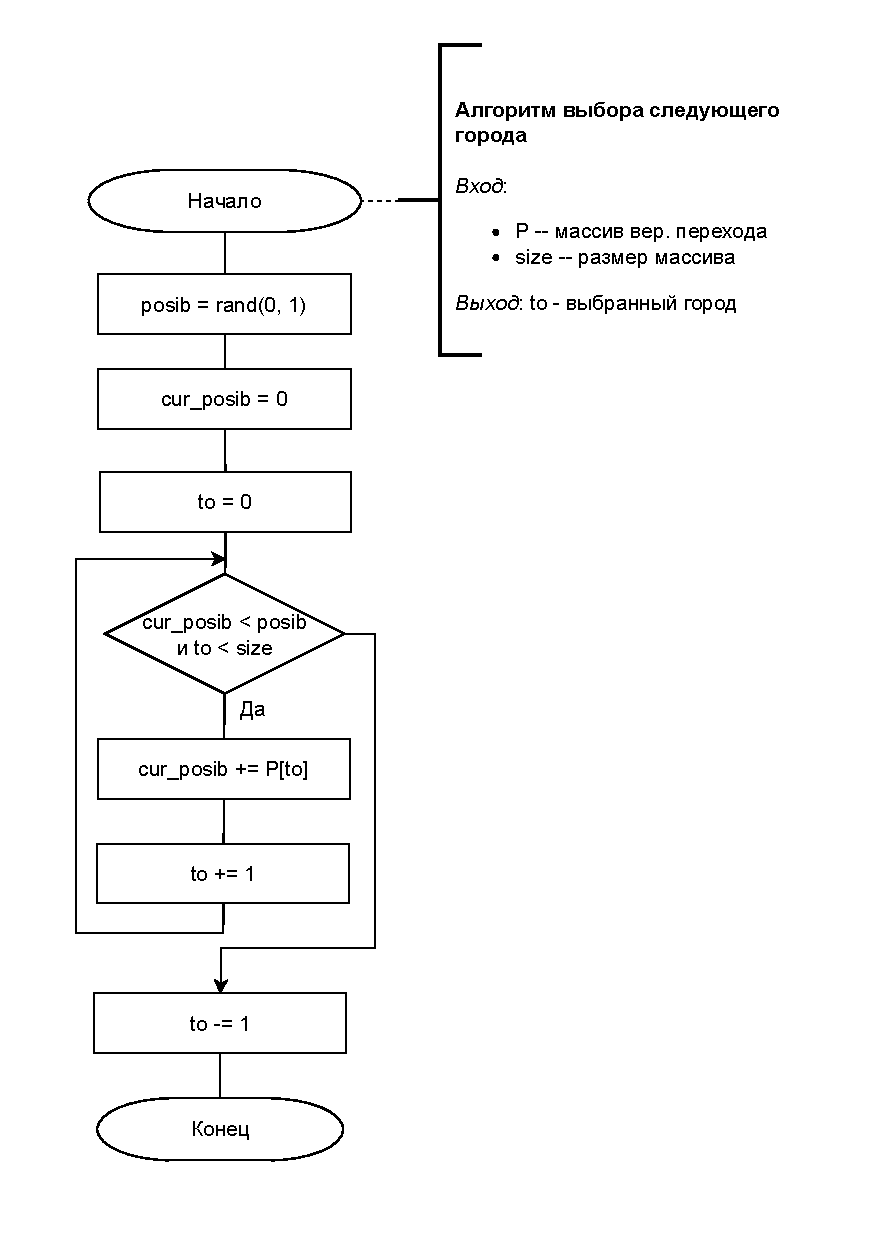
\includegraphics[scale=0.7]{img/cnl.pdf}
	\end{center}
	\captionsetup{justification=centering}
	\caption{Алгоритм выбора следующего города}
	\label{img:choose}
\end{figure}

\begin{figure}[H]
	\begin{center}
		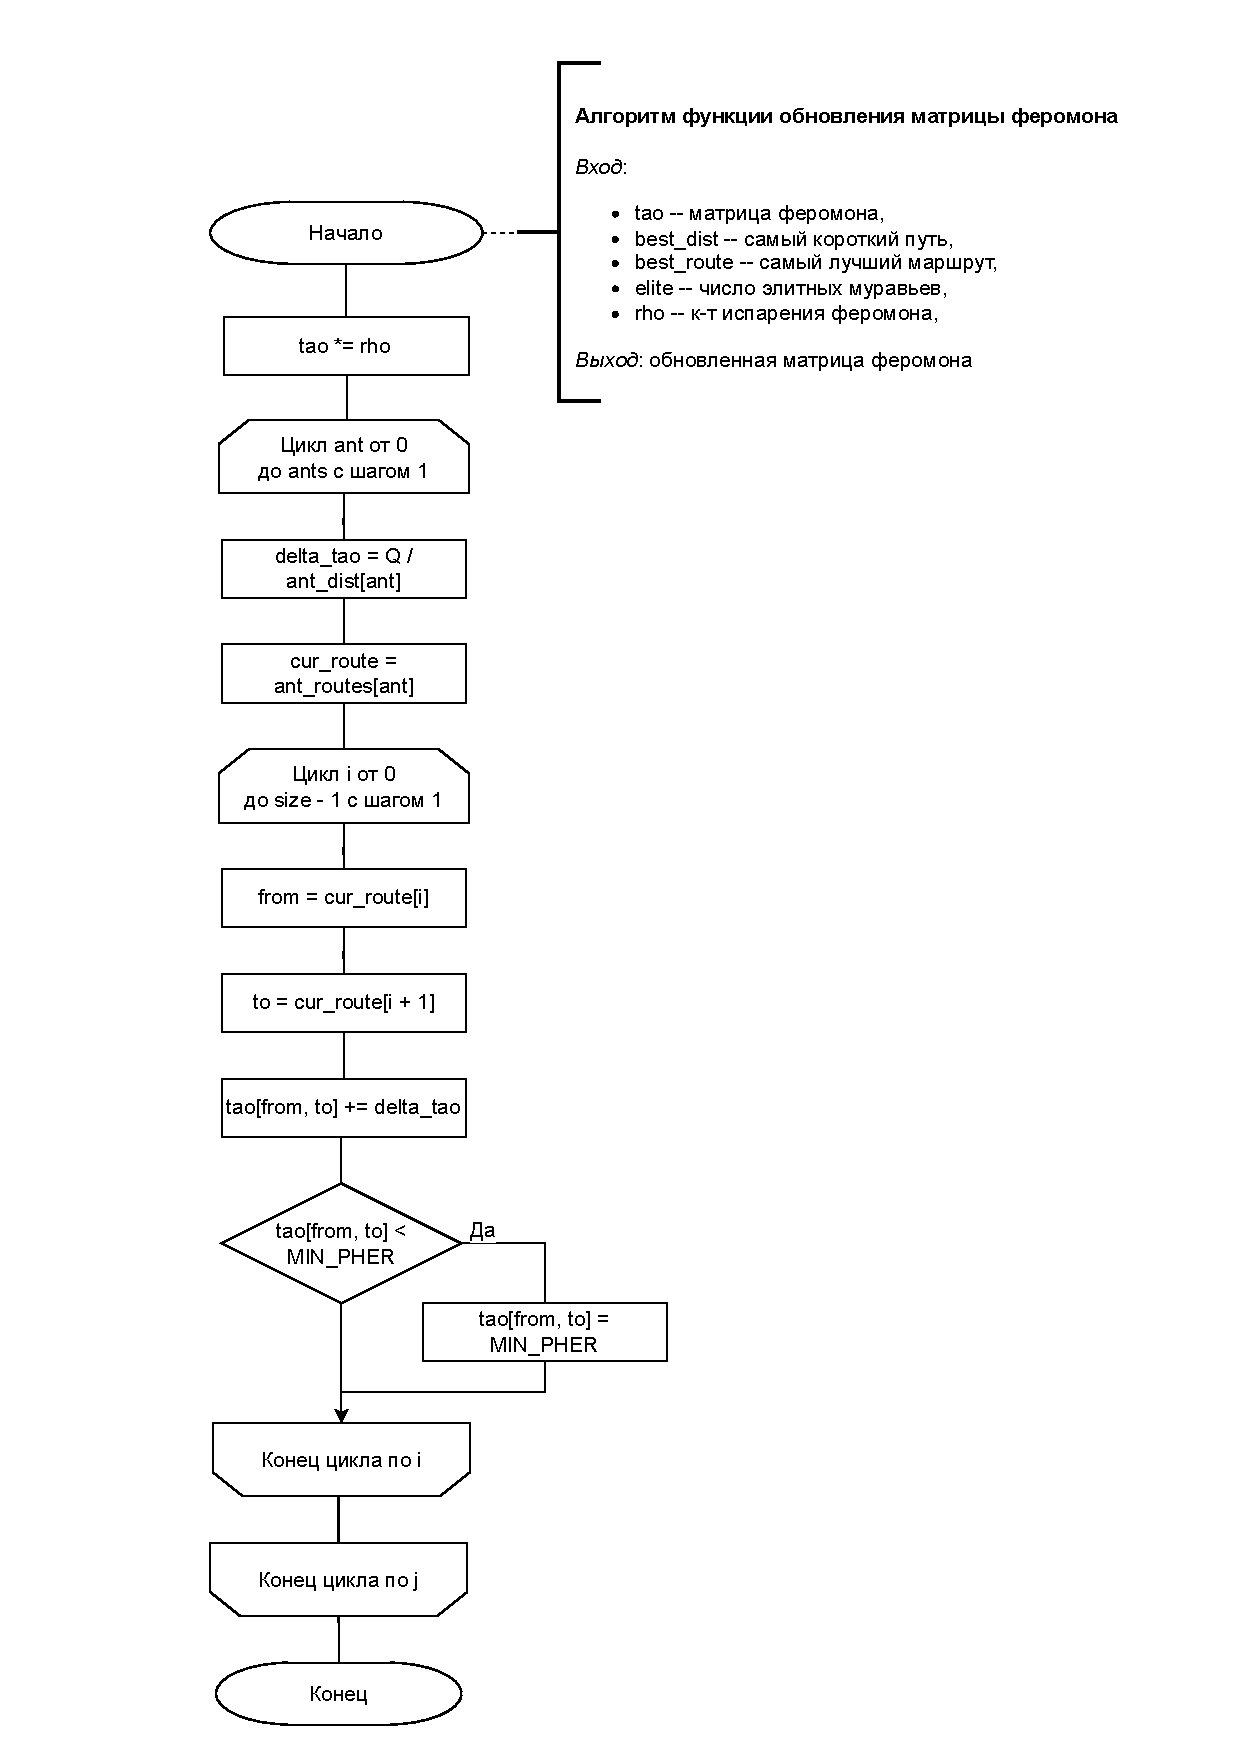
\includegraphics[scale=0.7]{img/up_pher.pdf}
	\end{center}
	\captionsetup{justification=centering}
	\caption{Алгоритм обновления феромона}
	\label{img:update}
\end{figure}

\section{Описание используемых типов и структур данных}

Для задания параметров $\alpha$, $\beta$ и коэффициента $\rho$ - тип данных $float$.

Структура данных - матрица - представляет собой двумерный список значений типа $float$.


\section{Вывод}

Были представлены схемы поиска оптимального пути, проходящего через все города по одному разу. Были указаны типы и структуры данных, используемые для реализации.

\chapter{Технологическая часть}
\hspace{\parindent}В данном разделе будут рассмотрены средства реализации, а также представлены листинги реализаций алгоритма линейной обработки данных и алгоритма конвейерной обработки данных.

\section{Средства реализации}
\hspace{\parindent}В данной работе для реализации был выбран язык программирования C++. Его возможностей достаточно для измерения процессорного времени и реализации алгоритмов.


\hspace{\parindent}Время работы было замерено с помощью функции
system\_clock::now()\cite{proc-time} из библиотеки std::chrono.


\section{Реализация алгоритмов}
\hspace{\parindent}В листингах \ref{lst:linear}-\ref{lst:conveyor} представлены реализации алгоритмов линейной и конвейерной обработки даных.
\clearpage

\begin{center}
	\captionsetup{skip=0pt,justification=raggedright,singlelinecheck=off}
    \begin{lstlisting}[label=lst:linear,language=Python, caption=Алгоритм линейной обработки данных]
void linear_execution(int count, size_t size, bool is_print)
{
	time_now = 0;
	for (int i = 0; i < count; i++)
	{
		matrix_t matrix = matrix_generate(size);
		matrix.det = matrix_determinant(matrix, 0, matrix.size, 1);
		matrix_dump(matrix);
	}
}
    \end{lstlisting}
\end{center}


\begin{center}
	\captionsetup{skip=0pt,justification=raggedright,singlelinecheck=off}
    \begin{lstlisting}[label=lst:conveyor,language=Python,caption=Алгоритм конвейерной обработки данных]
void parallel_execution(int count, size_t size)
{
	std::queue<int> q1;
	std::queue<matrix_t> q2;
	std::queue<matrix_t> q3;
	queues_t queues = {.q1 = q1, .q2 = q2, .q3 = q3};
	for (int i = 0; i < count; i++)
		q1.push(size);
	std::thread threads[3];
	threads[0] = std::thread(stage1_parallel, std::ref(q1), std::ref(q2), std::ref(q3));
	threads[1] = std::thread(stage2_parallel, std::ref(q1), std::ref(q2), std::ref(q3));
	threads[2] = std::thread(stage3_parallel, std::ref(q1), std::ref(q2), std::ref(q3));
	for (int i = 0; i < 3; i++)
		threads[i].join();
}
\end{lstlisting}
\end{center}
\clearpage

\begin{center}
	\captionsetup{skip=0pt,justification=raggedright,singlelinecheck=off}
	\begin{lstlisting}[label=lst:gen,language=Python,caption=Алгоритм генерации квадратной матрицы]
matrix_t matrix_generate(size_t size)
{
	std::vector<std::vector<int>> tmp_data;
	tmp_data.resize(size);
	for (size_t i = 0; i < size; i++)
	tmp_data[i].resize(size);
	matrix_t matrix;
	matrix.size = size;
	matrix.data = tmp_data;
	matrix.det = 0;
	for (size_t i = 0; i < matrix.size; i++)
	for (size_t j = 0; j < matrix.size; j++)
	matrix.data[i][j] = std::experimental::randint(1, 10);
	return matrix;
}
	\end{lstlisting}
\end{center}
\begin{center}
	\captionsetup{skip=0pt,justification=raggedright,singlelinecheck=off}
	\begin{lstlisting}[label=lst:det,language=Python,caption=Алгоритм вычисления детерминанта матрицы]
int matrix_determinant(matrix_t &matrix, int start, int end, int newDegree)
{
	int det = 0;
	int degree = newDegree;
	int size = matrix.size;
	if(size == 1)
	return matrix.data[0][0];
	else if(size == 2)
	return matrix.data[0][0]*matrix.data[1][1] - matrix.data[0][1]*matrix.data[1][0];
	else
	{
		for(int j = start; j < end; j++)
		{
			matrix_t copy = matrix_copy(matrix);
			matrix_WithoutRowAnColumn(copy, 0, j);
			det += degree * matrix.data[0][j] * matrix_determinant(copy, 0, copy.size, 1);;
			degree = -degree;
		}
	}
	return det;
}
	\end{lstlisting}
\end{center}
\clearpage
\begin{center}
\captionsetup{skip=0pt,justification=raggedright,singlelinecheck=off}
\begin{lstlisting}[label=lst:dump,language=Python,caption=Алгоритм записи матрицы и детерминанта в файл]
void matrix_dump(matrix_t matrix)
{
	ofstream logf(LOG, ios::app);
	if (logf.is_open())
	{
		for (size_t i = 0; i < matrix.size; i++)
		{
			for (size_t j = 0; j < matrix.size; j++)
			logf << matrix.data[i][j] << " ";
			logf << "\n";
		}
		logf << "\n\nDet: " << matrix.det << "\n----------\n";
		logf.close();
	}
}
\end{lstlisting}
\end{center}

\section{Функциональные тесты}
\hspace{\parindent}В таблице  \ref{tbl:testing} представлены функциональные тесты для программы.
\begin{table}[h]
	\begin{center}
		\captionsetup{skip=0pt,justification=raggedright,singlelinecheck=off}
		\caption{Функциональные тесты}
		\label{tbl:testing}
		\begin{tabular}{|c|c|c|c|}
			\hline
			Матрица & Линейная & Конвейерная & Эталон\\
			\hline
			 $\begin{pmatrix}
				0 & 1 & 2\\
				1 & 0 & 3\\
				2 & 4 & 0
			\end{pmatrix}$ &
			14 &
			14 &
			14 \\
			\hline
			$\begin{pmatrix}
				4 & 7 & 2 & 1 & 4\\
				4 & 2 & 3 & 5 & 2\\
				4 & 3 & 7 & 9 & 1\\
				3 & 7 & 9 & 2 & 9\\
				7 & 9 & 3 & 1 & 7
			\end{pmatrix}$ &
			-867 & -867 & -867 \\
			\hline
			$\begin{pmatrix}
				1 & 3 & 2 & 2\\
				7 & 4 & 2 & 5\\
				4 & 6 & 1 & 4\\
				2 & 6 & 9 & 7
			\end{pmatrix}$ &
			71 & 71 & 71 \\
			\hline
		\end{tabular}	
	\end{center}
\end{table}
\chapter{Исследовательская часть}
\hspace{\parindent}В данном разделе будет проведен сравнительный анализ алгоритмов по времени выполнения в зависимости от количества матриц и их размеров.

\section{Технические характеристики}
\hspace{\parindent}Технические характеристики устройства, на котором выполнялось тестирование представлены далее:

\begin{enumerate}
    \item операционная система: Windows 10 pro;
    \item память: 32 Гб;
    \item процессор: 12h Gen Intel(R) Core(TM) i5-12400 2.50 Ггц.
\end{enumerate}
\hspace{\parindent}Во время замеров компьютер был включен в сеть электропитания и был нагружен только системными программами и программой замеров.
\clearpage

\section{Демонстрация работы программы}
\hspace{\parindent}На рис. \ref{fig:demonstration} представлена демонстрация работы программы. 

\begin{figure}[h]
	\centering
	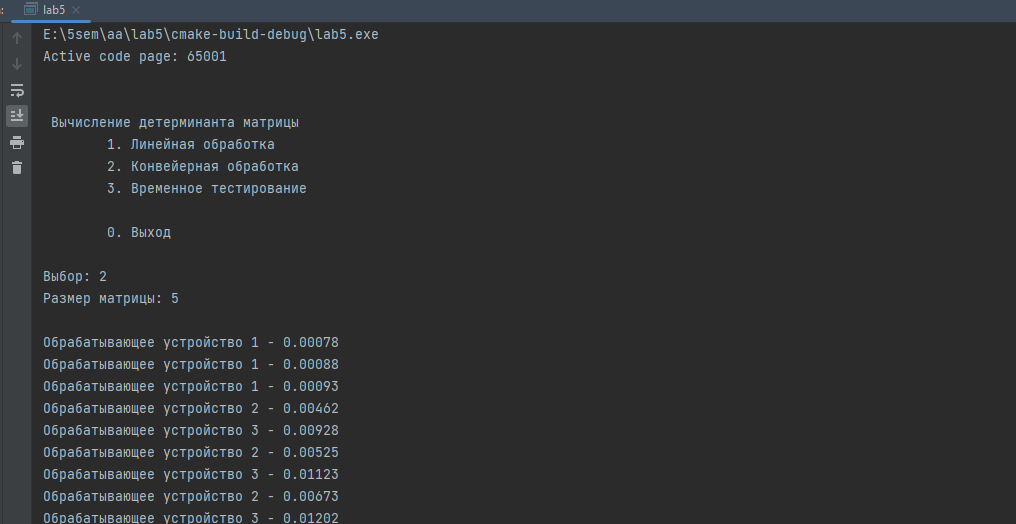
\includegraphics[height=0.5\textheight]{img/ex.png}
	\caption{Демонстрация работы программы}
	\label{fig:demonstration}
\end{figure}

\clearpage
\section{Время выполнения алгоритмов}
\hspace{\parindent}Результаты замеров приведены в таблицах \ref{tbl:time1}-\ref{tbl:time4}. Время указано в секундах.

\begin{table}[h]
    \begin{center}
    	\centering
    	\captionsetup{skip=0pt,justification=raggedright,singlelinecheck=off}
        \caption{Результаты замеров по времени для матриц размером 7}
        \label{tbl:time1}
        \begin{tabular}{|r|r|r|}
            \hline
            Количество матриц & Линейная & Конвейерная\\
           \hline
           1 & 0.0109 & 0.0118 \\
           \hline
           2 & 0.0223 & 0.0231 \\
           \hline
           3 & 0.0294 & 0.0331 \\
           \hline
           4 & 0.0430 & 0.0378 \\
           \hline
		\end{tabular}
	\end{center}
\end{table}
\begin{table}[h]
	\begin{center}
		\centering
		\captionsetup{skip=0pt,justification=raggedright,singlelinecheck=off}
		\caption{Результаты замеров по времени для матриц размером 8}
		\label{tbl:time2}
		\begin{tabular}{|r|r|r|}
			\hline
			Количество матриц & Линейная & Конвейерная\\
			\hline
			1 & 0.0815 & 0.0495 \\
			\hline
			2 & 0.1555 & 0.0940 \\
			\hline
			3 & 0.2385 & 0.1402 \\
			\hline
			4 & 0.3259 & 0.1944 \\
			\hline
		\end{tabular}
	\end{center}
\end{table}
\begin{table}[h]
	\begin{center}
		\centering
		\captionsetup{skip=0pt,justification=raggedright,singlelinecheck=off}
		\caption{Результаты замеров по времени для матриц размером 9}
		\label{tbl:time3}
		\begin{tabular}{|r|r|r|}
			\hline
			Количество матриц & Линейная & Конвейерная\\
			\hline
			1 & 0.7050 & 0.4097 \\
			\hline
			2 & 1.4126 & 0.8191 \\
			\hline
			3 & 2.1326 & 1.2208 \\
			\hline
			4 & 2.8180 & 1.5875 \\
			\hline
		\end{tabular}
	\end{center}
\end{table}
\begin{table}[H]
	\begin{center}
		\centering
		\captionsetup{skip=0pt,justification=raggedright,singlelinecheck=off}
		\caption{Результаты замеров по времени для матриц размером 10}
		\label{tbl:time4}
		\begin{tabular}{|r|r|r|}
			\hline
			Количество матриц & Линейная & Конвейерная\\
			\hline
			1 & 7.0369 & 3.6058 \\
			\hline
			2 & 14.1037 & 7.1952 \\
			\hline
			3 & 21.2308 & 10.6358 \\
			\hline
			4 & 28.1996 & 14.8571 \\
			\hline
		\end{tabular}
	\end{center}
\end{table}
\centerchapter{Заключение}
\hspace{\parindent}В результате было определено, что конвейерная обработка данных работает быстрее при размере матрицы равном 7 и количестве матриц от 4-х. Начиная с размера матрицы равного 8-ми, конвейерная обработка работает быстрее, чем линейная обработка.

\hspace{\parindent}Цель, лабораторной работы была достигнута, была исследована конвейерная обработка данных.

В ходе выполнения лабораторной работы были решены следующие задачи:
\begin{enumerate}
	\item описан и реализован алгоритм конвейерной обработки данных;
	\item реализован алгоритм линейной обработки данных;
	\item проведено тестирование по времени для этих алгоритмов;
	\item проведен сравнительный анализ по времени для этих алгоритмов.
\end{enumerate}
\addcontentsline{toc}{chapter}{Список использованных источников}
\renewcommand\bibname{Список использованных источников}
\bibliographystyle{utf8gost705u}
\bibliography{sources.bib}
\end{document}